\newlength\mystoreparindent
\newenvironment{myparindent}[1]{%
\setlength{\mystoreparindent}{\the\parindent}
\setlength{\parindent}{#1}
}{%
\setlength{\parindent}{\mystoreparindent}
}

\documentclass[a4paper]{article}
\usepackage{amssymb}
\usepackage{amsthm}
\usepackage{mathtools}
\usepackage{enumitem}
\usepackage{graphicx}
\usepackage{mathrsfs}
\usepackage{amsmath}

\DeclarePairedDelimiterX{\infdivx}[2]{(}{)}{%
  #1\;\delimsize\|\;#2%
}
\newcommand{\infdiv}{D\infdivx}
\DeclarePairedDelimiter{\norm}{\lVert}{\rVert}

\newtheorem{theorem}{Theorem}[section]
\newtheorem{corollary}{Corollary}[theorem]
\newtheorem{lemma}[theorem]{Lemma}

\graphicspath{ {./} }

\begin{document}

\begin{myparindent}{0pt}

Kyle Kloberdanz \newline
Math 417

\textbf{Exercise 3.1.4}:
Prove that a nonempty set $G$ with an associative operation $*$ is a group if
and only if the equations $g * x = h$ and $x * g = h$ have solutions in $G$
for all $g, h \in G$. \textit{Hint: Prove that if $e * g = g$ for some g, then
$e * h = h$ for all $h \in G$. Now appeal to Exercise 3.1.3} \newline

\textit{Note:} you should \textit{not} assume that the same $x$ solves both
equations simultaneously. In other words, prove that $G$ is a group if and only
if $*$ is an associative operation such that: \newline

for all $g, h \in G$ there exist $x, y \in G$ such that $g * x = h$ and $y * g = h$.
\newline

\textbf{Exercise 3.2.1}:
Suppose $n \ge 2$ is an integer and $d, d' > 0$ are two divisors of $n$. Prove
that $\langle [d] \rangle < \langle [d'] \rangle$ if and only if $d'|d$.
\newline

\begin{proof}
Let's start by assuming that $\langle [d] \rangle < \langle [d'] \rangle$.
Let $x, n \in \mathbb{Z}$.

\[ \langle [d] \rangle < \langle [d'] \rangle \implies [d] = \langle [d'] \rangle \implies [d] = [d']^x \implies [d]_n = [d']_n^x \implies \]
\[ d \equiv d'x \pmod n \implies d' | d \]

Working backwards:

\[ d' | d \implies d \equiv d'x \pmod n \implies [d]_n = [d']_n^x \implies [d] = [d']^x \implies \]
\[ [d] = \langle [d'] \rangle \implies \langle [d] \rangle < \langle [d'] \rangle \]
\end{proof}

\textbf{Exercise 3.2.2}:
Prove that the number of elements of order $n$ in $\mathbb{Z}_n$ is exactly
$\varphi(n)$, the Euler phi function of $n$.

\textit{Hint: You need to decide which $[a] \in \mathbb{Z}_n$ generate $\mathbb{Z}_n$}.
\newline

\textit{Note:} The group operation in $\mathbb{Z}_n$ is $+$ (modular addition)
\newline

\begin{proof}
  Recall, an equivalency class $[a]_n = \{ a + nk | k \in \mathbb{Z} \}$
  Recall that $1 = gcd(a, n) \iff 1 = ma + nk$ where $a, m, k \in \mathbb{Z}$.
  Because the generator for the integer is $\langle 1 \rangle$, we need to have
  some $a$ where $a + nk = [a + 1]$. If $gcd(a, n) \neq 1$, then we would be in
  a situation where there is no $a$ such that $a + nk = [a + 1]$, which would
  imply that this particular $a$ could not be a generator of $\mathbb{Z}_n$.
  Hence the only generators of $\mathbb{Z}_n$ are the elements of $\mathbb{Z}_n$
  that are relatively prime with $n$. The cardinality of this set is defined as
  $\varphi(n)$, therefore the number of elements of order $n$ in $\mathbb{Z}_n$
  is exactly $\varphi(n)$, the Euler phi function of $n$.
\end{proof}

\textbf{Exercise 3.2.3}
Draw the subgroup lattice for the groups
$\mathbb{Z}_8, \mathbb{Z}_{15}, \mathbb{Z}_{24}$, and $\mathbb{Z}_{30}$.
\newline

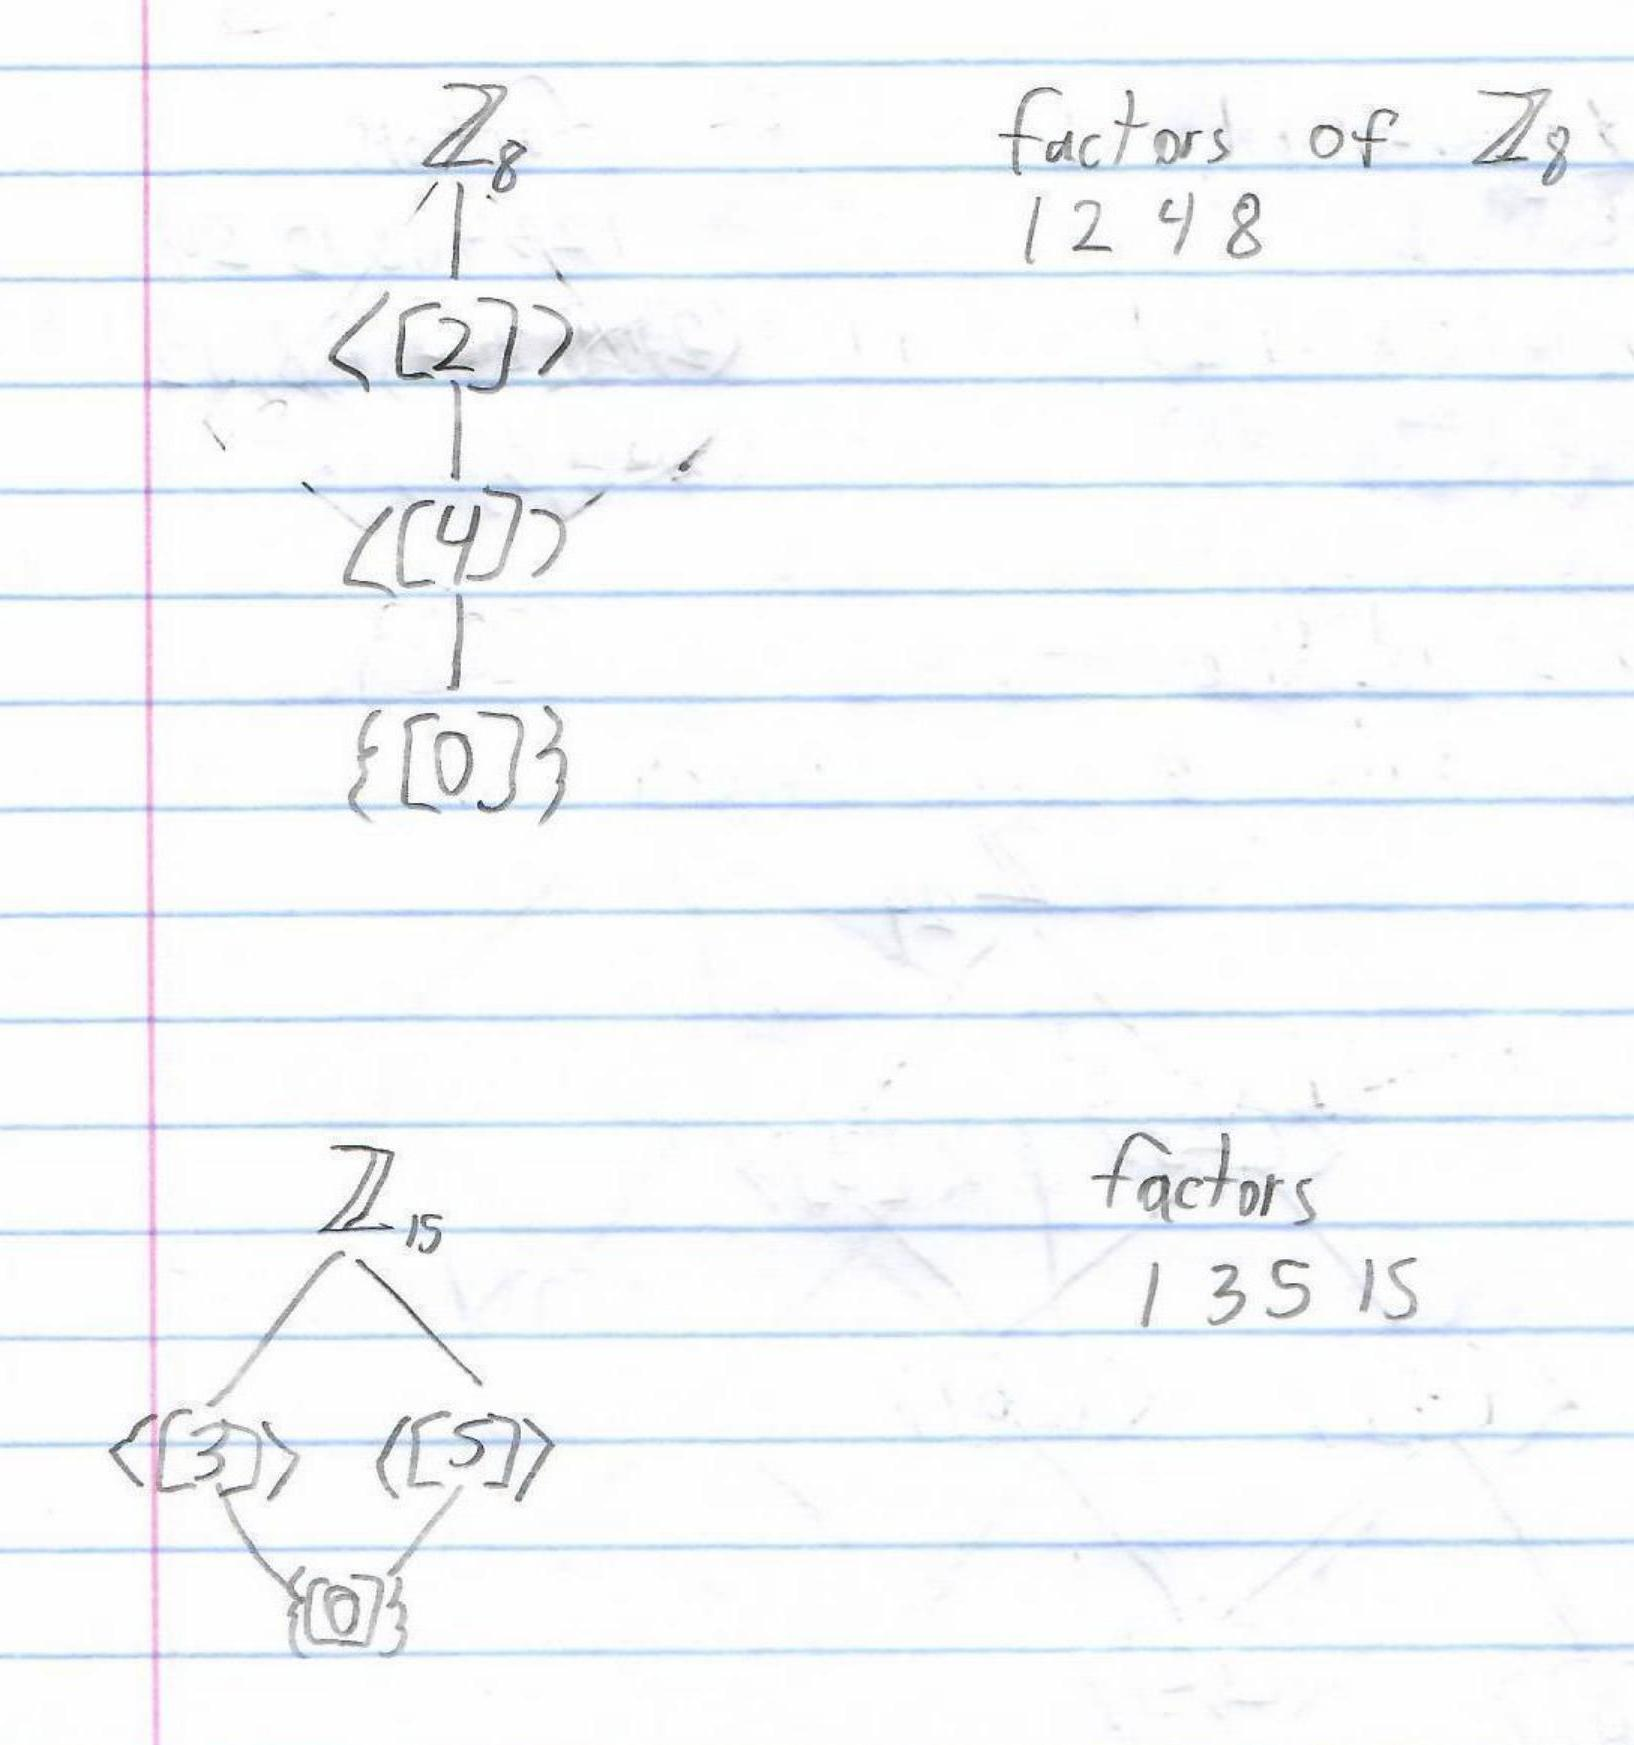
\includegraphics{lattice-Z8-Z15}
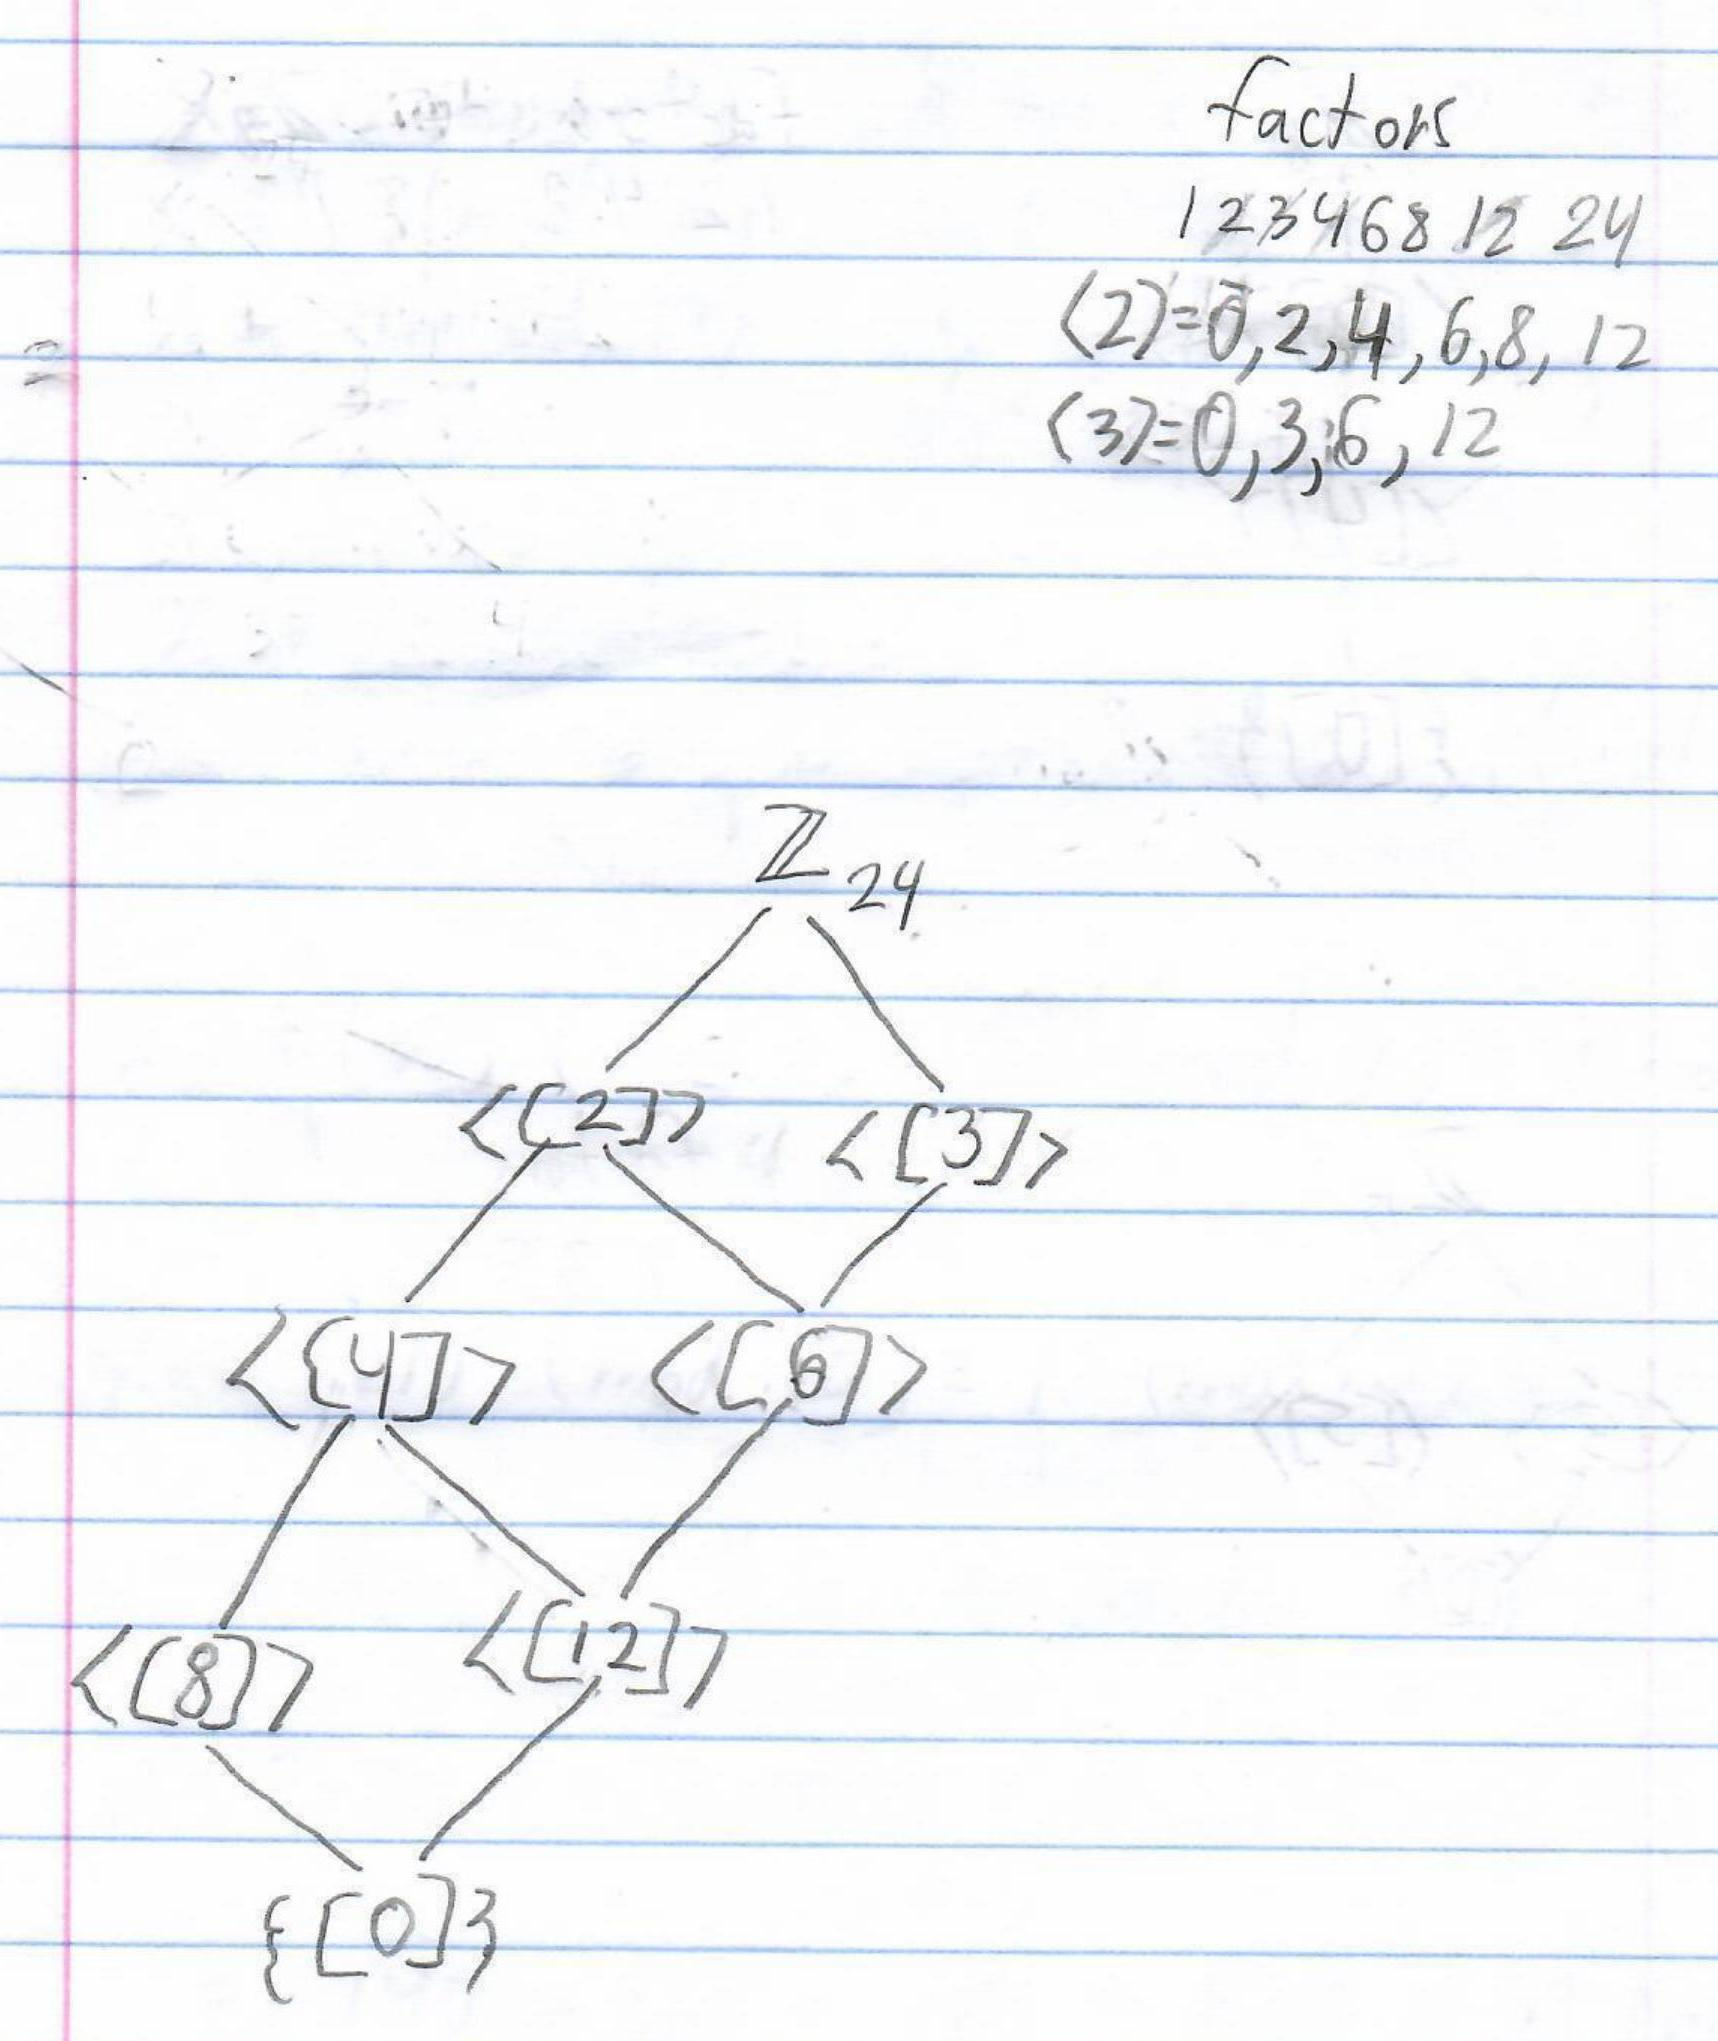
\includegraphics{lattice-Z24}
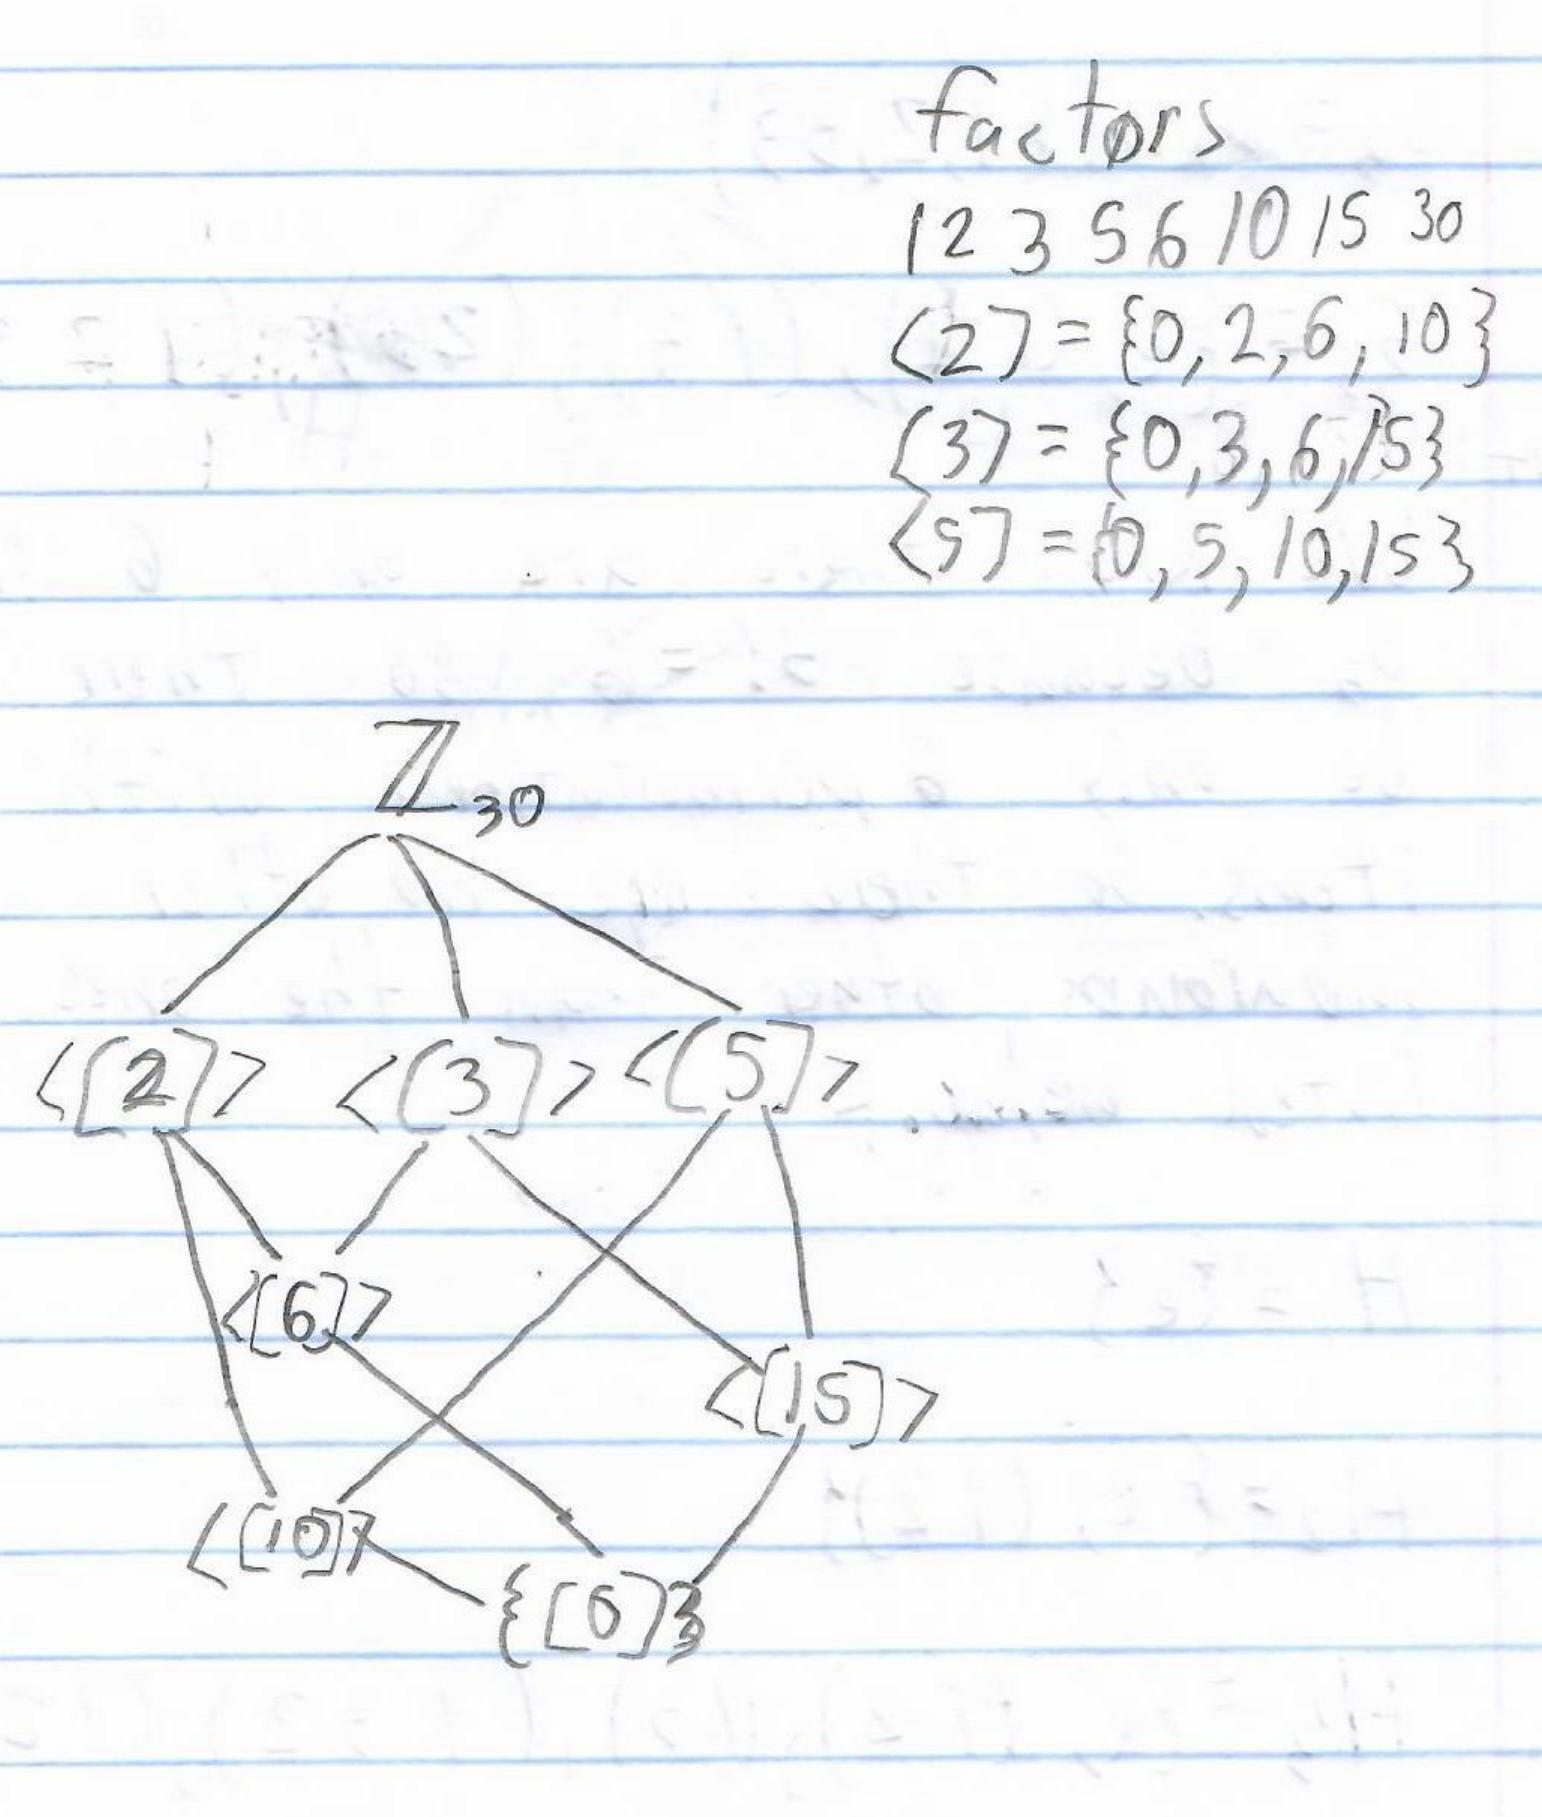
\includegraphics{lattice-Z30}

\textbf{Exercise 3.2.4}
Draw the subgroup lattice for $S_3$ (a group with respect to composition $\circ$).
You will need to find all the subgroups $H < S_3$ by hand (because we don't yet
have any theorems that tell us what the subgroups of $S_3$ are).
\textit{Hint: There are exactly 6 subgroups, but you should verify this by proving
that there are no other subgroups than the ones you have listed.}
\newline

To start, we will find the subgroups. \newline

Recall, any subgroup will have the following properties:
\begin{enumerate}
  \item Each group will contain the identity, $e$
  \item For all $g, h \in H$, $g * h \in H$
  \item For all $g \in H$, $g^{-1} \in H$
\end{enumerate}

Hence, each of the subgroups we find for $S_3$ must also have these properties.
To put this in plain English, each group we find will include the identity, it
will include the product of every other member of the group, and it will also
include the inverse of every member of the group. \newline

Recall from section 1.3 on permutations that $S_n = \textit{Sym}({1..n})$, so we
can use this definition to write $S_3$ as $\textit{Sym}(\{1, 2, 3\})$. \newline

We can expand out these symmetries into the set

\[ S_3 = \{e, (2 ~3), (1 ~2), (1 ~2 ~3), (1 ~3 ~2), (1 ~3) \} \]

As we can see, there are six elements in this set, which if we remember back to
probability and statistics classes, this makes sense because the number of
permutations of $3$ distinct items is $3! = 3 \times 2 \times 1 = 6$ permutations. \newline

We can also employ the powerful CAS system, Sage Mathematics, to automate this task.
\begin{verbatim}
sage: G = SymmetricGroup(3)
sage: {i for i in G}
{(), (2,3), (1,2), (1,2,3), (1,3,2), (1,3)}
\end{verbatim}

We will now find each of the subgroups, $H$, of this symmetry set. \newline

Let's begin with $H_1 = \{e\}$, the set that only contains the inverse. Let's
verify the three properties listed above. Notice that for the sake of brevity,
I will exclude repeats when verifying below. For example, I show that
$e \circ e = e \in H_1$, therefore we know that this will hold for $H_1$
through $H_6$, and therefore does not need to be shown each time. \newline

\begin{enumerate}
  \item $e \in H_1$
  \item $e \circ e = e \in H_1$
  \item $e \circ e = e \in H_1$
\end{enumerate}

Let $H_2 = \{e, (2 ~3)\}$.

\begin{enumerate}
  \item $e \in H_2$
  \item
  \[ e \circ (2 ~3) = (2 ~3) \circ e = (2 ~3) \in H_2 \]
  And
  \[ (2 ~3) \circ (2 ~3) = e \in H_2 \]
  \item $(2 ~3) \circ (2 ~3) = e \in H_2$
\end{enumerate}

Let $H_3 = \{e, (1 ~2)\}$.

\begin{enumerate}
  \item $e \in H_3$
  \item
  \[ e \circ (1 ~2) = (1 ~2) \circ e = (1 ~2) \in H_3 \]
  And
  \[ (1 ~2) \circ (1 ~2) = e \in H_3 \]
  \item $(1 ~2) \circ (1 ~2) = e \in H_3$
\end{enumerate}

Let $H_4 = \{e, (1 ~3)\}$.

\begin{enumerate}
  \item $e \in H_4$
  \item
  \[ e \circ (1 ~3) = (1 ~3) \circ e = (1 ~3) \in H_4 \]
  And
  \[ (1 ~3) \circ (1 ~3) = e \in H_4 \]
  \item $(1 ~3) \circ (1 ~3) = e \in H_4$
\end{enumerate}

Let $H_5 = \{e, (1 ~2 ~3), (1 ~3 ~2) \}$.

\begin{enumerate}
  \item $e \in H_5$
  \item
  \[ e \circ (1 ~2 ~3) = (1 ~2 ~3) \circ e = (1 ~2 ~3) \in H_5 \]
  And
  \[ e \circ (1 ~3 ~2) = (1 ~3 ~2) \circ e = (1 ~3 ~2) \in H_5 \]
  And
  \[ (1 ~3 ~2) \circ (1 ~2 ~3) = e \in H_5 \]
  And
  \[ (1 ~2 ~3) \circ (1 ~3 ~2) = e \in H_5 \]
  And
  \[ (1 ~2 ~3) \circ (1 ~2 ~3) = (3 ~1 ~2) \in H_5 \]
  And
  \[ (1 ~3 ~2) \circ (1 ~3 ~2) = (1 ~2 ~3) \in H_5 \]

  \item
  \[ (1 ~3 ~2) \circ (1 ~2 ~3) = e \in H_5 \]
  And
  \[ (1 ~2 ~3) \circ (1 ~3 ~2) = e \in H_5 \]
\end{enumerate}

Now the for this beast, $H_6 = \{ e, (2 ~3), (1 ~2), (1 ~2 ~3), (1 ~3 ~2), (1 ~3) \}$
\newline

To satisfy property 1, we see that $e \in H_6$.

We arrive at $H_6$ by the procedure below.
\begin{enumerate}
  \item Start with another set, for example $H_2$. We will see later on that we
  can start with any of our $H$ sets from above, and this procedure will still
  work.
  \item Append another item from $S_3$ into $H_6$.
  \item Calculate to composition of that element by each element already in
  $H_6$ and append that element into $H_6$.
  \item Repeat step 3 until the composition of every item has been calculated
  and appended to $H_6$.
\end{enumerate}

By following the procedure above, we construct $H_6$, which interestingly enough
happens to also be $S_3$. This procedure will satisfy property 2. \newline

From the calculations for $H_1$ through $H_5$, we have already worked out the
inverses of each element of $H_6$, and we can see that for any element of $H_6$
that the inverse is also present in $H_6$. \newline

By following this procedure starting with any set $H$ as our starting set, we
will construct the same set $H_6$ each and every time. Therefore, we have shown
that there are precisely six subgroups of $S_3$, because by appending any other
element of $S_3$ to sets $H_2$ through $H_5$ and following this procedure, we
only ever construct $H_6$. \newline

Therefore, our six subgroups of $S_3$ are:

\[ H_1 = \{e\} \]
\[ H_2 = \{e, (2 ~3)\} \]
\[ H_3 = \{e, (1 ~2)\} \]
\[ H_4 = \{e, (1 ~3)\} \]
\[ H_5 = \{e, (1 ~2 ~3), (1 ~3 ~2) \} \]
\[ H_6 = \{ e, (2 ~3), (1 ~2), (1 ~2 ~3), (1 ~3 ~2), (1 ~3) \} \]

The lattice drawing can be found below:

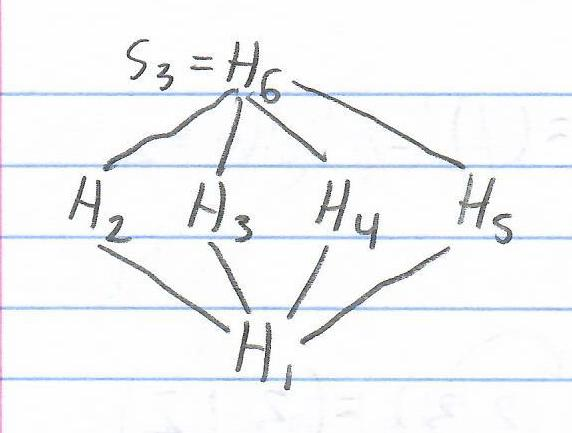
\includegraphics{lattice-S3} \newline

\textbf{Exercise 3.2.5}
Prove that if $G$ and $H$ are groups and $K < G$, $J < H$ are subgroups, then
$K \times J \subset G \times H$ is a subgroup. Construct an example of a
subgroup of $\mathbb{Z}_2 \times \mathbb{Z}_2$ which is \textbf{not} of the form
$K \times J$ for some $K < \mathbb{Z}_2$ and $J < \mathbb{Z}_2$.

\begin{proof}
  First we will show that $K \times J \subset G \times H$. Let $k \in K$,
  $j \in J$, $g \in G$, and $h \in H$. Because $K < G$ and $J < H$, $k \in G$
  and $j \in H$ for all $k$ and $j$, hence for any $k$, $j$, $g$, and $h$,
  $(k, j) \subset (g, h)$. \newline

  Second, we must show that for all $(k_1, j_1), (k_2, j_2) \in K \times J$ that
  $(k_1, j_1)(k_2, j_2) \in K \times J$.
  \[ (k_1, j_1)(k_2, j_2) = (k_1 k_2, j_1 j_2) \]

  Because $K$ and $J$ are subgroups, $k_1 k_2 \in K$ and $j_1 j_2 \in J$, hence
  $(k_1 k_2, j_1 j_2) \in K \times J$. \newline

  Third, we must show that for all $(k, j) \in K \times J$ that
  $(k, j)^{-1} \in K \times J$.

  \[ (k, j)(k, j)^{-1} = (k, j)(k^{-1}, j^{-1}) = (kk^{-1}, jj^{-1}) = (e, e) \]

  Verification:
  \[ (e, e)(k, j) = (ke, je) = (k, j) = (ek, ej) = (k, j)(e, e) \]

  Because $K$ and $J$ are subgroups, $k^{-1} \in K$ and $j^{-1} \in J$.
  Hence $(k^{-1}, j^{-1}) \in K \times J$, which is the inverse of $K \times J$.
  \newline

  Because of these three reasons, $K \times J \subset G \times H$ is a subgroup,
  so therefore we can write:

  \[ K \times J < G \times H \]
\end{proof}

\end{myparindent}
\end{document}
